\section{Display Driver}
\begin{frame}{Display Timing}
	\begin{center}
		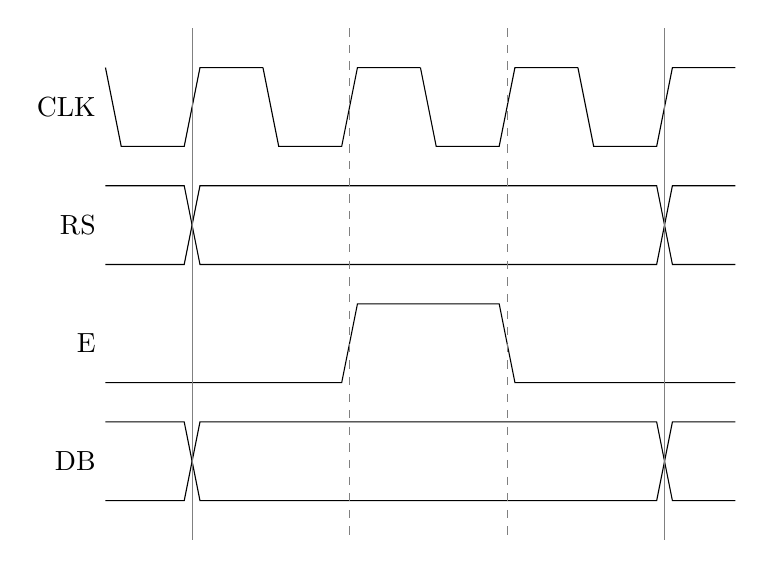
\begin{tikzpicture}
			\foreach \x in {0,2,4,6} \draw (\x-0.1,1) -- (\x+0.1,0) -- (\x+0.9,0) -- (\x+1.1,1) -- (\x+1.9,1);
			\draw (-0.1,-1.5) -- (0.9,-1.5) -- (1.1,-0.5) -- (6.9,-0.5) -- (7.1,-1.5) -- (7.9,-1.5);
			\draw (-0.1,-0.5) -- (0.9,-0.5) -- (1.1,-1.5) -- (6.9,-1.5) -- (7.1,-0.5) -- (7.9,-0.5);

			\draw (-0.1,-3.0) -- (2.9,-3.0) -- (3.1,-2.0) -- (4.9,-2.0) -- (5.1,-3.0) -- (7.9,-3.0);

			\draw (-0.1,-4.5) -- (0.9,-4.5) -- (1.1,-3.5) -- (6.9,-3.5) -- (7.1,-4.5) -- (7.9,-4.5);
			\draw (-0.1,-3.5) -- (0.9,-3.5) -- (1.1,-4.5) -- (6.9,-4.5) -- (7.1,-3.5) -- (7.9,-3.5);

			\node[left] at (-.1, 0.5) {CLK};
			\node[left] at (-.1,-1.0) {RS};
			\node[left] at (-.1,-2.5) {E};
			\node[left] at (-.1,-4.0) {DB};

			\draw[gray] (1,1.5) -- (1,-5);
			\draw[gray,dashed] (3,1.5) -- (3,-5);
			\draw[gray,dashed] (5,1.5) -- (5,-5);
			\draw[gray] (7,1.5) -- (7,-5);
		\end{tikzpicture}
	\end{center}
\end{frame}

\begin{frame}{Display Driver Overview}
	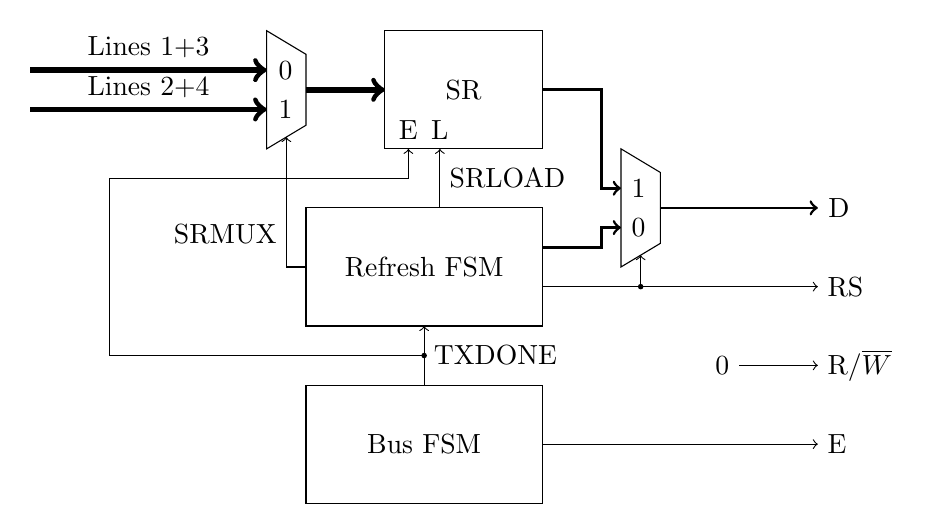
\begin{tikzpicture}
		\draw[line width=2pt,->] (0,0) -> (3, 0) node[midway,above] {Lines 1+3} node[right] {0};
		\draw[line width=2pt,->] (0,-.5) -> (3, -.5) node[midway,above] {Lines 2+4} node[right] {1};
		\draw[line width=2pt,->] (3.5,-.25) -> (4.5,-.25);
		\draw[line width=1pt,->] (6.5,-.25) -- (7.25,-.25) -- (7.25,-1.5) -> (7.5,-1.5) node[right] {1};
		\draw[line width=1pt,->] (6.5,-2.25) -- (7.25,-2.25) -- (7.25,-2) -> (7.5,-2) node[right] {0};
		\draw[line width=1pt,->] (8,-1.75) -> (10,-1.75) node[right] {D};

		\draw (3,.5) -- (3.5,.2) -- (3.5,-.7) -- (3,-1) -- cycle;

		\node at (5.5, -.25) {SR};
		\draw (4.5,.5) rectangle (6.5,-1);

		\node at(5,-2.5) {Refresh FSM};
		\draw (3.5,-1.75) rectangle (6.5,-3.25);

		\node at(5,-4.75) {Bus FSM};
		\draw (3.5,-4) rectangle (6.5,-5.5);

		\draw[->] (5,-4) -> (5,-3.25) node[right,midway] {TXDONE};
		\draw[->] (5,-3.625) -- (1,-3.625) -- (1,-1.375) -- (4.8, -1.375) -> (4.8, -1) node[above] { E };
		\fill (5,-3.625) circle (1pt);

		\draw[->] (3.5,-2.5) -- (3.25,-2.5) -> (3.25,-.85) node[left,near start] {SRMUX};

		\draw[->] (5.2,-1.75) -> (5.2,-1) node[above] {L} node[midway,right] {SRLOAD};

		\draw (7.5,-1.0) -- (8,-1.3) -- (8,-2.2) -- (7.5,-2.5) -- cycle;

		\draw[->] (6.5,-2.75) -> (10,-2.75) node[right] {RS};
		\draw[->] (7.75,-2.75) -> (7.75,-2.35);
		\fill (7.75,-2.75) circle (1pt);
		\draw[->] (6.5,-4.75) -> (10,-4.75) node[right] {E};
		\draw[->] (9,-3.75) node[left] {0} -> (10,-3.75) node[right] {R/$\overline{\text{W}}$};
	\end{tikzpicture}
\end{frame}

\begin{frame}{Display Driver Bus FSM}
	\begin{center}
		\begin{tikzpicture}[every state/.style={text width=1.3cm,align=center,node distance=.5cm},font=\tiny,auto]
			\node at (2,1.2) {All transitions occur on CLK$\uparrow$};
			\node[state] (S0) at (0.0,0) { \textbf{S0} \\ E = 0 \\ TXDONE = 0 };
			\node[state] (S1) at (4.0,0) { \textbf{S1} \\ E = 1 \\ TXDONE = 0 };
			\node[state] (S2) at (-60:4) { \textbf{S2} \\ E = 0 \\ TXDONE = 1 };

			\path[->] (S0) edge (S1)
						 (S1) edge (S2)
						 (S2) edge (S0)
						 (S0) ++ (-30:2) edge (S0);
		\end{tikzpicture}
	\end{center}
\end{frame}

\begin{frame}{Display Driver Refresh FSM}
	\begin{center}
		\begin{tikzpicture}[every state/.style={text width=1.3cm,align=center,node distance=.5cm},font=\tiny,auto]
			\node at (4,1.5) {All transitions occur on CLK$\uparrow$ if TXDONE = 1};
			\node[state]                       (FunctionSet)  { \textbf{INIT0} \\ RS = 0 \\ D = 0x38 \\ SRMUX = X \\ SRLOAD = X };
			\node[state,right=of FunctionSet]  (DisplayOnOff) { \textbf{INIT1} \\ RS = 0 \\ D = 0x0C \\ SRMUX = X \\ SRLOAD = X };
			\node[state,right=of DisplayOnOff] (SetAddrUpper) { \textbf{LOAD0} \\ RS = 0 \\ D = 0x80 \\ SRMUX = 0 \\ SRLOAD = 1 };
			\node[state,right=of SetAddrUpper] (WriteUpper)   { \textbf{SEND0} \\ RS = 1 \\ D = X    \\ SRMUX = X \\ SRLOAD = 0 };
			\node[state,below=of WriteUpper]   (SetAddrLower) { \textbf{LOAD1} \\ RS = 0 \\ D = 0xC0 \\ SRMUX = 0 \\ SRLOAD = 1 };
			\node[state,left =of SetAddrLower] (WriteLower)   { \textbf{SEND1} \\ RS = 1 \\ D = X    \\ SRMUX = X \\ SRLOAD = 0 };

			\path[->] (FunctionSet) ++(0,-2) edge (FunctionSet)
						 (FunctionSet)  edge                                  (DisplayOnOff)
						 (DisplayOnOff) edge                                  (SetAddrUpper)
						 (SetAddrUpper) edge                                  (WriteUpper)
						 (WriteUpper)   edge             node {SRDONE = 1}    (SetAddrLower)
											 edge[loop right,near start,above] node {SRDONE = 0} ()
						 (SetAddrLower) edge                                  (WriteLower)
						 (WriteLower)   edge             node {SRDONE = 1}    (SetAddrUpper)
											 edge[loop left]  node {SRDONE = 0}    ();
			\path[->,dashed]
						 (WriteLower)   edge                                  (FunctionSet);
		\end{tikzpicture}
	\end{center}
\end{frame}

\section{Time Buffer}
\begin{frame}{Time Buffer Circuit}
	\begin{center}
		\begin{tikzpicture}
			\tikzset{dcf update/.style={}}
			\tikzset{dcf update fill/.style={}}
			\tikzset{counter update/.style={}}
			\tikzset{counter update fill/.style={}}
			\only<2> {
				\tikzset{dcf update/.style={color=red}}
				\tikzset{dcf update fill/.style={fill=red}}
			}
			\only<3> {
				\tikzset{counter update/.style={color=red}}
				\tikzset{counter update fill/.style={fill=red}}
			}

			\node[rectangle,draw=black,minimum height=0.75cm,minimum width=4cm,above right] at (0,-1) {+ 1 min, valid <= 0};
			\node[rectangle,draw=black,minimum height=2.75cm,minimum width=1cm,above right] at (2,-4) {};
			\node[rectangle,draw=black,minimum height=0.75cm,minimum width=1cm,above right] at (0,-3.5) {$\geq 1$};
			\node[rectangle,draw=black,minimum height=0.75cm,minimum width=1cm,above right] at (-.25,-5.5) {$\geq 1$};
			\node[rectangle,draw=black,minimum height=0.75cm,minimum width=2.25cm,above right] at (1,-5.5) {counter};
			\node[rectangle,draw=black,minimum height=0.75cm,minimum width=2.75cm,above right] at (3.5,-5.5) {= 59999};

			\draw (.75,-1.25) -- (1.25,-1.50) -- (1.25,-2.25) -- (.75,-2.50) -- cycle;

			% time signals
			\draw[red!50!black,line width=2pt,->,counter update] (0,-0.625) -- (-.25,-0.625) -- (-.25,-1.666667) -> (.75,-1.666667) node[right,black,counter update] {0};
			\draw[red!50!black,line width=2pt,->,dcf update] (-1,-2.083333) node[left,black] {DCF77\_dec} -> (.75,-2.083333) node[right,black,dcf update] {1};
			\draw[red!50!black,line width=2pt,->, dcf update,counter update] (1.25,-1.875) -> (2,-1.875) node[right,black,dcf update,counter update] {D};
			\draw[red!50!black,line width=2pt,->] (4.25,-1.875) -- (7,-1.875);
			\draw[red!50!black,line width=2pt,->,counter update] (3,-1.875) node[left,black] {Q} -- (4.25,-1.875) -- (4.25,-.625) -> (4,-.625);

			% OR gate outputs
			\draw[->,dcf update,counter update] (1,-3.125) -> (2,-3.125) node[right] {E};
			\draw[->,dcf update,counter update] (1.5,-3.125) -- (1.5,-3.75) -- (-.5,-3.75) -- (-.5,-5) -> (-.25,-5);
			\fill[dcf update fill,counter update fill] (1.5,-3.125) circle (1pt);
			\draw[->,dcf update,counter update] (.75,-5.125) -> (1,-5.125) node[right] {R};
			\draw[->] (-.75,-4.25) -- (-.75,-5.25) -> (-.25,-5.25);

			% OR gate / MUX inputs
			\fill[dcf update fill] (-.25,-2.083333) circle (1pt);
			\draw[->,dcf update] (-.25,-2.083333) -- (-.25,-3) -> (0,-3);
			\draw[->,dcf update] (-.25,-2.625) -- (1,-2.625) -> (1,-2.375);
			\fill[dcf update fill] (-.25,-2.625) circle (1pt);
			\draw[->,counter update] (6.25,-5.125) -- (6.5,-5.125) -- (6.5,-4.5) -- (-.25,-4.5) -- (-.25,-3.25) -- (0,-3.25);

			% counter value
			\draw[->,line width=2pt] (3.25,-5.125) -> (3.5,-5.125);

			% clock and reset lines
			\draw[white!50!black,line width=2pt] (-1,-4.25) node[left,black] {clk, reset} -- (3.25,-4.25);
			\draw[->] (2.333333,-4.25) -- (2.333333,-4) node[above] {R};
			\draw[->] (2.666667,-4.25) -- (2.666667,-4);
			\draw (2.666667,-4) +(0.173205,0) -- +(0,.2) -- +(-0.173205,0);
			\draw[->] (3,-4.25) ->  (3,-4.75);
			\draw (3,-4.75) +(0.173205,0) -- +(0,-.2) -- +(-0.173205,0);
			\fill (2.333333,-4.25) circle (1pt);
			\fill (2.666667,-4.25) circle (1pt);
			\fill (3,-4.25) circle (1pt);
			\fill (-.75,-4.25) circle (1pt);

		\end{tikzpicture}
	\end{center}
\end{frame}

\end{document}
